
%% bare_conf.tex
%% V1.3
%% 2007/01/11
%% by Michael Shell
%% See:
%% http://www.michaelshell.org/
%% for current contact information.
%%
%% This is a skeleton file demonstrating the use of IEEEtran.cls
%% (requires IEEEtran.cls version 1.7 or later) with an IEEE conference paper.
%%
%% Support sites:
%% http://www.michaelshell.org/tex/ieeetran/
%% http://www.ctan.org/tex-archive/macros/latex/contrib/IEEEtran/
%% and
%% http://www.ieee.org/

%%*************************************************************************
%% Legal Notice:
%% This code is offered as-is without any warranty either expressed or
%% implied; without even the implied warranty of MERCHANTABILITY or
%% FITNESS FOR A PARTICULAR PURPOSE! 
%% User assumes all risk.
%% In no event shall IEEE or any contributor to this code be liable for
%% any damages or losses, including, but not limited to, incidental,
%% consequential, or any other damages, resulting from the use or misuse
%% of any information contained here.
%%
%% All comments are the opinions of their respective authors and are not
%% necessarily endorsed by the IEEE.
%%
%% This work is distributed under the LaTeX Project Public License (LPPL)
%% ( http://www.latex-project.org/ ) version 1.3, and may be freely used,
%% distributed and modified. A copy of the LPPL, version 1.3, is included
%% in the base LaTeX documentation of all distributions of LaTeX released
%% 2003/12/01 or later.
%% Retain all contribution notices and credits.
%% ** Modified files should be clearly indicated as such, including  **
%% ** renaming them and changing author support contact information. **
%%
%% File list of work: IEEEtran.cls, IEEEtran_HOWTO.pdf, bare_adv.tex,
%%                    bare_conf.tex, bare_jrnl.tex, bare_jrnl_compsoc.tex
%%*************************************************************************

% *** Authors should verify (and, if needed, correct) their LaTeX system  ***
% *** with the testflow diagnostic prior to trusting their LaTeX platform ***
% *** with production work. IEEE's font choices can trigger bugs that do  ***
% *** not appear when using other class files.                            ***
% The testflow support page is at:
% http://www.michaelshell.org/tex/testflow/



% Note that the a4paper option is mainly intended so that authors in
% countries using A4 can easily print to A4 and see how their papers will
% look in print - the typesetting of the document will not typically be
% affected with changes in paper size (but the bottom and side margins will).
% Use the testflow package mentioned above to verify correct handling of
% both paper sizes by the user's LaTeX system.
%
% Also note that the "draftcls" or "draftclsnofoot", not "draft", option
% should be used if it is desired that the figures are to be displayed in
% draft mode.
%
%\documentclass[conference]{IEEEtran}
\documentclass[conference,a4paper]{IEEEtran}
% Add the compsoc option for Computer Society conferences.
%
% If IEEEtran.cls has not been installed into the LaTeX system files,
% manually specify the path to it like:
% \documentclass[conference]{../sty/IEEEtran}





% Some very useful LaTeX packages include:
% (uncomment the ones you want to load)


% *** MISC UTILITY PACKAGES ***
%
%\usepackage{ifpdf}
% Heiko Oberdiek's ifpdf.sty is very useful if you need conditional
% compilation based on whether the output is pdf or dvi.
% usage:
% \ifpdf
%   % pdf code
% \else
%   % dvi code
% \fi
% The latest version of ifpdf.sty can be obtained from:
% http://www.ctan.org/tex-archive/macros/latex/contrib/oberdiek/
% Also, note that IEEEtran.cls V1.7 and later provides a builtin
% \ifCLASSINFOpdf conditional that works the same way.
% When switching from latex to pdflatex and vice-versa, the compiler may
% have to be run twice to clear warning/error messages.






% *** CITATION PACKAGES ***
%
%\usepackage{cite}
% cite.sty was written by Donald Arseneau
% V1.6 and later of IEEEtran pre-defines the format of the cite.sty package
% \cite{} output to follow that of IEEE. Loading the cite package will
% result in citation numbers being automatically sorted and properly
% "compressed/ranged". e.g., [1], [9], [2], [7], [5], [6] without using
% cite.sty will become [1], [2], [5]--[7], [9] using cite.sty. cite.sty's
% \cite will automatically add leading space, if needed. Use cite.sty's
% noadjust option (cite.sty V3.8 and later) if you want to turn this off.
% cite.sty is already installed on most LaTeX systems. Be sure and use
% version 4.0 (2003-05-27) and later if using hyperref.sty. cite.sty does
% not currently provide for hyperlinked citations.
% The latest version can be obtained at:
% http://www.ctan.org/tex-archive/macros/latex/contrib/cite/
% The documentation is contained in the cite.sty file itself.






% *** GRAPHICS RELATED PACKAGES ***
%
\ifCLASSINFOpdf
  \usepackage[pdftex]{graphicx}
  % declare the path(s) where your graphic files are
  % \graphicspath{{../pdf/}{../jpeg/}}
  % and their extensions so you won't have to specify these with
  % every instance of \includegraphics
  % \DeclareGraphicsExtensions{.pdf,.jpeg,.png}
\else
  % or other class option (dvipsone, dvipdf, if not using dvips). graphicx
  % will default to the driver specified in the system graphics.cfg if no
  % driver is specified.
  % \usepackage[dvips]{graphicx}
  % declare the path(s) where your graphic files are
  % \graphicspath{{../eps/}}
  % and their extensions so you won't have to specify these with
  % every instance of \includegraphics
  % \DeclareGraphicsExtensions{.eps}
\fi
% graphicx was written by David Carlisle and Sebastian Rahtz. It is
% required if you want graphics, photos, etc. graphicx.sty is already
% installed on most LaTeX systems. The latest version and documentation can
% be obtained at: 
% http://www.ctan.org/tex-archive/macros/latex/required/graphics/
% Another good source of documentation is "Using Imported Graphics in
% LaTeX2e" by Keith Reckdahl which can be found as epslatex.ps or
% epslatex.pdf at: http://www.ctan.org/tex-archive/info/
%
% latex, and pdflatex in dvi mode, support graphics in encapsulated
% postscript (.eps) format. pdflatex in pdf mode supports graphics
% in .pdf, .jpeg, .png and .mps (metapost) formats. Users should ensure
% that all non-photo figures use a vector format (.eps, .pdf, .mps) and
% not a bitmapped formats (.jpeg, .png). IEEE frowns on bitmapped formats
% which can result in "jaggedy"/blurry rendering of lines and letters as
% well as large increases in file sizes.
%
% You can find documentation about the pdfTeX application at:
% http://www.tug.org/applications/pdftex





% *** MATH PACKAGES ***
%
\usepackage[cmex10]{amsmath}
% A popular package from the American Mathematical Society that provides
% many useful and powerful commands for dealing with mathematics. If using
% it, be sure to load this package with the cmex10 option to ensure that
% only type 1 fonts will utilized at all point sizes. Without this option,
% it is possible that some math symbols, particularly those within
% footnotes, will be rendered in bitmap form which will result in a
% document that can not be IEEE Xplore compliant!
%
% Also, note that the amsmath package sets \interdisplaylinepenalty to 10000
% thus preventing page breaks from occurring within multiline equations. Use:
%\interdisplaylinepenalty=2500
% after loading amsmath to restore such page breaks as IEEEtran.cls normally
% does. amsmath.sty is already installed on most LaTeX systems. The latest
% version and documentation can be obtained at:
% http://www.ctan.org/tex-archive/macros/latex/required/amslatex/math/





% *** SPECIALIZED LIST PACKAGES ***
%
%\usepackage{algorithmic}
% algorithmic.sty was written by Peter Williams and Rogerio Brito.
% This package provides an algorithmic environment fo describing algorithms.
% You can use the algorithmic environment in-text or within a figure
% environment to provide for a floating algorithm. Do NOT use the algorithm
% floating environment provided by algorithm.sty (by the same authors) or
% algorithm2e.sty (by Christophe Fiorio) as IEEE does not use dedicated
% algorithm float types and packages that provide these will not provide
% correct IEEE style captions. The latest version and documentation of
% algorithmic.sty can be obtained at:
% http://www.ctan.org/tex-archive/macros/latex/contrib/algorithms/
% There is also a support site at:
% http://algorithms.berlios.de/index.html
% Also of interest may be the (relatively newer and more customizable)
% algorithmicx.sty package by Szasz Janos:
% http://www.ctan.org/tex-archive/macros/latex/contrib/algorithmicx/




% *** ALIGNMENT PACKAGES ***
%
%\usepackage{array}
% Frank Mittelbach's and David Carlisle's array.sty patches and improves
% the standard LaTeX2e array and tabular environments to provide better
% appearance and additional user controls. As the default LaTeX2e table
% generation code is lacking to the point of almost being broken with
% respect to the quality of the end results, all users are strongly
% advised to use an enhanced (at the very least that provided by array.sty)
% set of table tools. array.sty is already installed on most systems. The
% latest version and documentation can be obtained at:
% http://www.ctan.org/tex-archive/macros/latex/required/tools/


%\usepackage{mdwmath}
%\usepackage{mdwtab}
% Also highly recommended is Mark Wooding's extremely powerful MDW tools,
% especially mdwmath.sty and mdwtab.sty which are used to format equations
% and tables, respectively. The MDWtools set is already installed on most
% LaTeX systems. The lastest version and documentation is available at:
% http://www.ctan.org/tex-archive/macros/latex/contrib/mdwtools/


% IEEEtran contains the IEEEeqnarray family of commands that can be used to
% generate multiline equations as well as matrices, tables, etc., of high
% quality.


%\usepackage{eqparbox}
% Also of notable interest is Scott Pakin's eqparbox package for creating
% (automatically sized) equal width boxes - aka "natural width parboxes".
% Available at:
% http://www.ctan.org/tex-archive/macros/latex/contrib/eqparbox/





% *** SUBFIGURE PACKAGES ***
%\usepackage[tight,footnotesize]{subfigure}
% subfigure.sty was written by Steven Douglas Cochran. This package makes it
% easy to put subfigures in your figures. e.g., "Figure 1a and 1b". For IEEE
% work, it is a good idea to load it with the tight package option to reduce
% the amount of white space around the subfigures. subfigure.sty is already
% installed on most LaTeX systems. The latest version and documentation can
% be obtained at:
% http://www.ctan.org/tex-archive/obsolete/macros/latex/contrib/subfigure/
% subfigure.sty has been superceeded by subfig.sty.



%\usepackage[caption=false]{caption}
%\usepackage[font=footnotesize]{subfig}
% subfig.sty, also written by Steven Douglas Cochran, is the modern
% replacement for subfigure.sty. However, subfig.sty requires and
% automatically loads Axel Sommerfeldt's caption.sty which will override
% IEEEtran.cls handling of captions and this will result in nonIEEE style
% figure/table captions. To prevent this problem, be sure and preload
% caption.sty with its "caption=false" package option. This is will preserve
% IEEEtran.cls handing of captions. Version 1.3 (2005/06/28) and later 
% (recommended due to many improvements over 1.2) of subfig.sty supports
% the caption=false option directly:
%\usepackage[caption=false,font=footnotesize]{subfig}
%
% The latest version and documentation can be obtained at:
% http://www.ctan.org/tex-archive/macros/latex/contrib/subfig/
% The latest version and documentation of caption.sty can be obtained at:
% http://www.ctan.org/tex-archive/macros/latex/contrib/caption/




% *** FLOAT PACKAGES ***
%
%\usepackage{fixltx2e}
% fixltx2e, the successor to the earlier fix2col.sty, was written by
% Frank Mittelbach and David Carlisle. This package corrects a few problems
% in the LaTeX2e kernel, the most notable of which is that in current
% LaTeX2e releases, the ordering of single and double column floats is not
% guaranteed to be preserved. Thus, an unpatched LaTeX2e can allow a
% single column figure to be placed prior to an earlier double column
% figure. The latest version and documentation can be found at:
% http://www.ctan.org/tex-archive/macros/latex/base/



%\usepackage{stfloats}
% stfloats.sty was written by Sigitas Tolusis. This package gives LaTeX2e
% the ability to do double column floats at the bottom of the page as well
% as the top. (e.g., "\begin{figure*}[!b]" is not normally possible in
% LaTeX2e). It also provides a command:
%\fnbelowfloat
% to enable the placement of footnotes below bottom floats (the standard
% LaTeX2e kernel puts them above bottom floats). This is an invasive package
% which rewrites many portions of the LaTeX2e float routines. It may not work
% with other packages that modify the LaTeX2e float routines. The latest
% version and documentation can be obtained at:
% http://www.ctan.org/tex-archive/macros/latex/contrib/sttools/
% Documentation is contained in the stfloats.sty comments as well as in the
% presfull.pdf file. Do not use the stfloats baselinefloat ability as IEEE
% does not allow \baselineskip to stretch. Authors submitting work to the
% IEEE should note that IEEE rarely uses double column equations and
% that authors should try to avoid such use. Do not be tempted to use the
% cuted.sty or midfloat.sty packages (also by Sigitas Tolusis) as IEEE does
% not format its papers in such ways.





% *** PDF, URL AND HYPERLINK PACKAGES ***
%
%\usepackage{url}
% url.sty was written by Donald Arseneau. It provides better support for
% handling and breaking URLs. url.sty is already installed on most LaTeX
% systems. The latest version can be obtained at:
% http://www.ctan.org/tex-archive/macros/latex/contrib/misc/
% Read the url.sty source comments for usage information. Basically,
% \url{my_url_here}.





% *** Do not adjust lengths that control margins, column widths, etc. ***
% *** Do not use packages that alter fonts (such as pslatex).         ***
% There should be no need to do such things with IEEEtran.cls V1.6 and later.
% (Unless specifically asked to do so by the journal or conference you plan
% to submit to, of course. )


% correct bad hyphenation here
\hyphenation{op-tical net-works semi-conduc-tor}


\begin{document}
%
% paper title
% can use linebreaks \\ within to get better formatting as desired
\title{Can we date an artist's work from catalogue photographs?}


% author names and affiliations
% use a multiple column layout for up to three different
% affiliations
\author{\IEEEauthorblockN{Alexander David Brown}
\IEEEauthorblockA{Computer Science,\\
Aberystwyth University,\\
Penglais,\\
Aberystwyth,\\
Ceredigion,\\
Wales SY23 3DB\\
adb9@aber.ac.uk}
\and
\IEEEauthorblockN{Gareth Lloyd Roderick}
\IEEEauthorblockA{School of Art,\\
Aberystwyth University,\\
Buarth Mawr,\\
Aberystwyth,\\
Wales SY23 1NG\\
glr7@aber.ac.uk}
\and
\IEEEauthorblockN{Hannah M. Dee\footnote{Corresponding Author}}
\IEEEauthorblockA{Computer Science,\\
Aberystwyth University,\\
Penglais,\\
Aberystwyth,\\
Ceredigion,\\
Wales SY23 3DB\\
hmd1@aber.ac.uk}
\and
\IEEEauthorblockN{Lorna M. Hughes}
\IEEEauthorblockA{The National Library of Wales,\\
Aberystwyth,\\
Ceredigion,\\
Wales SY23 3BU\\
lorna.hughes@llgc.org.uk}}

% conference papers do not typically use \thanks and this command
% is locked out in conference mode. If really needed, such as for
% the acknowledgment of grants, issue a \IEEEoverridecommandlockouts
% after \documentclass

% for over three affiliations, or if they all won't fit within the width
% of the page, use this alternative format:
% 
%\author{\IEEEauthorblockN{Michael Shell\IEEEauthorrefmark{1},
%Homer Simpson\IEEEauthorrefmark{2},
%James Kirk\IEEEauthorrefmark{3}, 
%Montgomery Scott\IEEEauthorrefmark{3} and
%Eldon Tyrell\IEEEauthorrefmark{4}}
%\IEEEauthorblockA{\IEEEauthorrefmark{1}School of Electrical and Computer Engineering\\
%Georgia Institute of Technology,
%Atlanta, Georgia 30332--0250\\ Email: see http://www.michaelshell.org/contact.html}
%\IEEEauthorblockA{\IEEEauthorrefmark{2}Twentieth Century Fox, Springfield, USA\\
%Email: homer@thesimpsons.com}
%\IEEEauthorblockA{\IEEEauthorrefmark{3}Starfleet Academy, San Francisco, California 96678-2391\\
%Telephone: (800) 555--1212, Fax: (888) 555--1212}
%\IEEEauthorblockA{\IEEEauthorrefmark{4}Tyrell Inc., 123 Replicant Street, Los Angeles, California 90210--4321}}




% use for special paper notices
%\IEEEspecialpapernotice{(Invited Paper)}




% make the title area
\maketitle


\begin{abstract}
%\boldmath
Kyffin Williams, art changes over time, blah blah blah. Features, colour, edges, histograms of oriented gradients; strong correlation using leave-one-out methodology.
Exemplars; artistic and statistic. 
\end{abstract}
% IEEEtran.cls defaults to using nonbold math in the Abstract.
% This preserves the distinction between vectors and scalars. However,
% if the conference you are submitting to favors bold math in the abstract,
% then you can use LaTeX's standard command \boldmath at the very start
% of the abstract to achieve this. Many IEEE journals/conferences frown on
% math in the abstract anyway.

% no keywords




% For peer review papers, you can put extra information on the cover
% page as needed:
% \ifCLASSOPTIONpeerreview
% \begin{center} \bfseries EDICS Category: 3-BBND \end{center}
% \fi
%
% For peerreview papers, this IEEEtran command inserts a page break and
% creates the second title. It will be ignored for other modes.
\IEEEpeerreviewmaketitle



\section{Introduction}
% no \IEEEPARstart
% You must have at least 2 lines in the paragraph with the drop letter
% (should never be an issue)

This paper presents a interdisciplinary computational study into the modelling
of artistic style, and how this style changes over time.  Sir John Kyffin
Williams (1918-2006) was one of the predominant figures in Welsh art of the
twentieth century.  Kyffin -- as he was almost universally known in Wales --
studied at the Slade School of Art and worked as an art master at Highgate
School, before returning to live on his native Anglesey in 1973.  He was a
prolific painter and once claimed to have painted ``two pictures per week when
in London, and three per week when in Wales.'\cite[p.209]{Williams1993Across}
With a career spanning from the mid-1940s to approximately 2004, this rate
amounts to a large body of work.

His style evolved from a very representational style to something more
expressive, which retained representational qualities: the computer scientists
on our team would say that the paintings became more \emph{blocky}; the art
historians that his landscapes are almost constructed with swathes of textural
paint. His was a style characterised by thick impasto paint, applied almost
exclusively with palette knife, although the application technique appears to
change over time. This development of style led us to wonder: is it possible to
date the pictures from images alone?

Through a collection of digital photographs of oil paintings, collected from
museum websites, catalogues and other sources, we first investigate whether it
is possible to date a painting based upon image features. We show that using a
K-nearest neighbour classifier, tested using a leave-one-out methodology, we
can obtain a strong correlation between image feature descriptors and year of
painting. We go on to investigate whether exemplar based methods are able to
improve on this, using what we call \emph{artistic exemplars} (paintings
selected by an expert as being typical for a particular year) and
\emph{statistic exemplars} (paintings which are near the centre of year-based
clusters in feature space).

%This paper presents a interdisciplinary computational study into the modelling
%of artistic style, and how this style changes over time. The artist Sir John
%(Kyffin) Williams painted from X to 2004, and produced a good many paintings
%during this period -- he was a prolific painter \cite{Harris2011How}. His style
%evolved from a very figurative, representational style, to something more
%abstract: the computer scientists on our team would say that the paintings
%became more \emph{blocky}; the art historians that \textbf{whatever lorna
%and lloyd want to say}.  Through a collection of digital photographs of oil
%paintings, collected from museum websites, catalogues and other sources, we
%first investigate whether it is possible to date a painting from an unknown
%year based upon image features alone.  We show that using a K-nearest neighbour
%classfier, tested using a leave-one-out methodology, we can obtain a strong
%correlation between image feature descriptors and year of painting. We go on to
%investigate whether exemplar based methods are able to improve on this, using
%what we call \emph{artistic} exemplars (paintings selected by an expert as
%being typical for a particular year) and \emph{statistic} exemplars (paintings
%which are near the centre of year-based clusters in feature space). 


\section{Background}
% 1 Page on Lloyd's work

Although also a portrait painter, Williams is primarily known for his landscape
paintings of north west Wales and Anglesey. While his technique and style
changed over the years, his landscapes in oil are instantly recognisable, often
featuring bold chunks of colour, and various points during his career bold
black outlines to figures and landscapes features. Greens, browns and greys
often form the palette of his paintings of the Welsh landscape. These colour
selections seem appropriate for the artist’s claim that melancholy, derived
from the ``dark hills, heavy clouds and enveloping sea mists'', is a national
characteristic of the Welsh.\cite{Williams1993Across} This combination of
colour selection and technique seems appropriate for the depiction of the areas
where he painted. Many of his most successful paintings are said to have a
``dark quality'' in depicting ``rain lashed hillsides,'' and it was this
darkness which ``makes his landscapes so distinctively
Welsh.''\cite{Davies2004100} 

%Both of the above descriptions could be applicable
%to paintings in the collections of the National Library of Wales such as
%Snowdonian Summits (1970-1990) or Yr Wyddfa a Grib Goch (1950-1960).

The aesthetic of Williams’s Welsh landscapes is contrasted by the paintings he
made following a trip to Patagonia to paint the landscape and people of the
Welsh communities there in 1968 as part of a Winston Churchill Foundation
scholarship. The colours and application of paint in pictures produced in
following this journey (such as \emph{Lle Cul}, \emph{Henry Roberts},
\emph{Bryngwyn Patagonia}, \emph{Euros Hughes Irrigating his Fields}, all 1969,
National Library of Wales) differ starkly from paintings of Welsh landscapes,
incorporating pinks, purples and oranges. This contrast, combined with the fact
that the Patagonian pictures were produced during a definite period of time has
reinforced our interest in the analysis of the formal qualities of pictures
from different collections remotely, using digital images. 

Williams’s work is well represented in public collections in Wales
(particularly at the National Library of Wales, the National Museums and
Galleries of Wales and Oriel Ynys M\^{o}n, Anglesey). His pictures, often
depicting the landscape and people of north-west Wales were also tremendously
popular with the art buying public. Of the 325 paintings by Williams in public
collections in the UK listed on the BBC/Public Catalogue Foundation's ``Your
Paintings'' website, 212 of them are in the collections of the National Library
of Wales\cite{2013Your}. Many of these paintings were bequeathed to the Library
as part of a larger bequest by the artist (including works on paper and other
archival material). Many of the pictures which came to the library from the
artist’s studio had little in the way of metadata, and as such have been
catalogued with large date-ranges estimating the dates of production.  This
uncertainty in metadata is another motivating force behind the current project.

%\textbf{We need here to mention key features of Kyffin's work, Patagonia, where he painted}

\subsection{Taking a digital humanities approach to art history}

Digital humanities is an established area of research that brings together
digital content, tools and methods in order to address and create new knowledge
across the disciplines. Digital humanities approaches can be seen in two
distinct types of inquiry. The first is to carry out \emph{traditional}
humanities research more effectively or efficiently, by applying computational
methods or approaches to digitized humanities sources (originally text, image,
or audio-visual content from archives or libraries). Using John Unsworth’s
definition of ``scholarly primitives''\cite{unsworth00} digital humanities
scholarship customarily involves the use of digital tools and methods for
discovering, annotating, comparing, referring, sampling, illustrating, or
representing humanities data. A classic example of this sort of work would be
the use of concordances and other computer-based analysis of digitized primary
sources that have been processed by optical character recognition software to
count, classify, or interpret digital texts (see, for example, the Historical
Concordance of the Welsh language\cite{welshconcordance}).  The second strand
of digital humanities inquiry is the development of new research questions that
can only be developed through the synthesis of digital content, tools and
methods: work that would have otherwise been unimaginable\cite{hughes11}. This
type of research is by necessity multi-disciplinary, drawing together expertise
to be found across humanities, scientific and engineering disciplines, as well
as involving content experts from libraries, archives and museums. However, in
order to be truly transformative, this type of research must also be
interdisciplinary. 

The National Library of Wales now has a research programme in digital
collections, which is a forum for investigation into the digital collections of
Wales in collaboration with academics and students at universities in Wales and
beyond, in order to develop new research based around the digital content
created by the Library \cite{llgc}. The research project described in this
article is an example of a digital humanities collaborative venture, bringing
together digital humanists, art historians, and computer scientists.  The
results of this research have value across all these groups. Arts historians
are able to better investigate a large corpus of digital paintings through the
application of computer science approaches to this content, and computer
scientists are able to configure new approaches in imaging to working with a
complex humanities data set. 

\subsection{Computer vision and the analysis of paintings}

%Stroke analysis is one of the main goals for this project. It is quite apparent from looking at 
%Kyffin Williams' paintings that his brush-strokes change over time, his early work having lots of
%smaller strokes over the canvas to large bold strokes in his later work.

\textbf{XXX Alex or Hannah are going to have to read \cite{Stork2009Computer}, cite it sensibly, and pull some other references which are relevant}

When we consider computer vision-based analysis of painterly style we find that
the vast majority of  work concentrates on brush stroke detection and analysis.
For example, Berezhnoy and colleagues in \cite{Berezhnoy2009Automatic} detect
brush-strokes by moving a circular filter across the whole painting to find the
ridges of strokes, then filling any unbroken areas. They then shrunk these
areas to a single pixel line and fitted a $n^{\text{th}}$ order polynomial to
this line.

Li et al \cite{Li2012Rhythmic} use a combination of edge analysis and
clustering in colour space to determine strokes; a number of heuristics
involving branching, stroke-width modeling, and gap filling are then used to
refine the original brush stroke estimates. One interesting element of this
work, from our perspective, is the ability to date some of Van Gogh's paintings
to a known period in his career.

Techniques based upon stroke analysis, whilst applicable to the work of some
artists, are not applicable to all. In particular, Kyffin Williams painted with
a palette knife and whilst there are clear \emph{strokes} identifiable in
his style, these vary widely in size and shape, so the morphological techniques
which can detect strokes in Van Gogh's work are unlikely to pay off when
considering the blockier paintings in the Williams oeuvre. Another difference
of note is that much work on computerised painting analysis (including
\cite{Li2012Rhythmic, Berezhnoy2009Automatic}) is based upon high resolution
scans acquired in controlled conditions, whereas the current paper deals
instead with a collection of photographs from catalogues, websites, and other
disparate sources. 

\section{The image dataset}

Our image dataset consists of 325 paintings, with associated metadata. Metadata
includes title, year or year ranges (for those works where year is unknown but
can be estimated by curators), genre, original painting size, painting
materials and image size.

These photographs of paintings are challenging in and of themselves: they are
not colour calibrated; some suffer from reflections (towards the end of his
life Kyffin painted using exceptionally thick and textural strokes, which gives
specularities on the catalogue images); they are at varying resolutions; and
come from a range of different cameras. Image size bears little relation to the
original painting size, and some images are even optimised for the web.
Table~\ref{summary_t} below summarises the dataset

\begin{table}[h]
\centering
\begin{tabular}{| l | c | c | p{3cm} |}
\hline
Type & Number & Number & Notes \\
  & & (Known date) &  \\
\hline
Landscapes  & 247 & 64 & \\
Portraits   &  52 & 35 & \\
Seascapes   &  11 &  2 & \\
Still lifes &   4 &  1 & \\
Other       &   8 &  0 & Other or studies \\
\hline
\end{tabular}
\vspace{0.5em}
\caption{A summary of our Kyffin Williams painting dataset}
\label{summary_t}
\end{table}

\textbf{XXX It may be worth putting in something here about image size vs painting size?}


\section{Methodology}
% 0.5 Page on the validation - LOOCV

Within our database of 325 paintings, we know the actual year of painting for
102 artworks. In order to determine the accuracy of our results, rather than
work with the full dataset (and work with images with uncertain metadata in the
form of date ranges), we have used a leave-one-out cross validation
methodology. This involves us taking a painting for which we know the year, and
then using our classifier to guess that year; thus we are able to tell whether
we are right. We are also able, if we are wrong, to determine exactly how wrong
we are.  

To simplify the classification stage we use a K-Nearest Neighbour (KNN)
classifier with the other 101 paintings for which we know the date. KNN is a
fast, non-parametric classifier which makes no assumptions about the underlying
patterns in the data, merely that paintings from around the same time will be
similarly located in our feature space(s). Whilst we suspect that there may be
some broader underlying trend in the change of style, for this work have
concentrated on features for classification rather than the question of
classification or regression itself. 
 
\begin{figure}
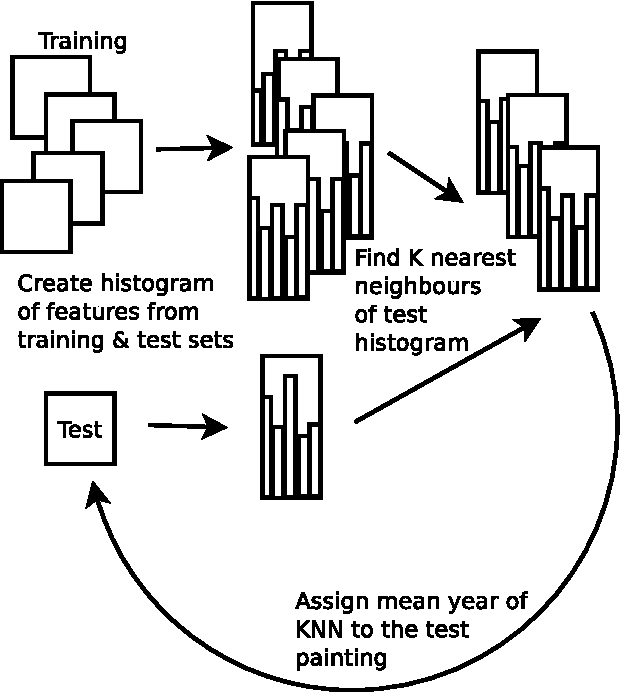
\includegraphics[width=8cm]{img/kyffin_overview.pdf}
\caption{Overview of the classification methodology}
\label{LOOCV}
\end{figure}

Thus for each feature set, we take all paintings for which we know the year of
creation; select one painting, and find its nearest neighbours within that
feature space. The year assigned by our classifier to that painting is the mean
of the K neighbours; we found this provided better results than both median and
mode.  Figure~\ref{LOOCV} provides an overview of this classification
methodology.

We also know that painting's actual year, and we can plot actual against
predicted year for all known-year paintings.  To measure goodness of fit, the
Pearson's product-moment correlation coefficient was calculated on these
orderings; this provides us with a performance measure of each classifier.  It
is also possible to test Pearson's R for statistical significance; thus
significance levels are reported alongside R in this paper.  With all of the
feature spaces we consider, it is possible treat the painting descriptors as
histograms.  This allows us to use a single distance measure, namely
chi-squared, in our K-nearest neighbour classification.

\section{An exploration of colour and texture features}

% 0.5 page on references
% 4 pages on the rest

The digital analysis of paintings is a broad reseach area. Within the
methodology we have selected, there are many feature spaces which could be
useful: from simple analysis of the way in which colour changes over time,
through edge detection, to texture analysis. We have concentrated on lower
level image features -- colours, textures, and edges -- rather than attempt to
extract brush strokes. As mentioned earlier, Williams painted with a pallette
knife rather than a brush, and his work is characterised by angularity rather
than identifiable ``strokes''.  In this section we describe the various feature
sets and feature spaces we have explored; results for each of these are
presented in Section~\ref{results} below.

There is a clear (to the eye) trend in colour usage, as the paintings get
``gloomier'' over time, so we started with simple colour-space analysis: taking
the mean RGB for each painting and using this with our KNN classfier; we also
tested other colour spaces, such as HSV. Promisingly this provided us with a
positive correlation. 
 
Staying with the colour variation theme, we then used colour histograms, which
provide a more precise representation of the way Kyffin Williams used colour.
These histograms were developed by counting the number of pixels within a
particular colour range for each painting, and then building a normalised
histogram representing the colour usage. 

\textbf{XXX Alex how many bins? }
 
As a lot of Kyffin Williams' paintings are highly textural, edge detection and
texture analysis was thought to be a good avenue to explore.  Firstly, we
investigated simple \emph{edginess}; as a rough estimate of the the edge
properties of the artworks we apply a Canny \cite{Canny1986Computational} edge
detector to the paintings, and then use a count of edge pixels as our feature. 

Texture analysis is a continuation of edge detection. Instead of taking simply
the strength and number of edges, we create a histogram of orientated gradients
as in \cite{Dalal2005Histograms}. In this way we begin to build up a richer
representation of the texture of a painting. Given the change in style of
Kyffin Williams' work, moving away from figurative representations with curved
lines towards more blocky rectilinear brush strokes, we expect these edge
orientation frequencies to change over time. To this end we used simple
steerable filters $S$, applied to the image at $0$, $\frac{\pi}{4}$,
$\frac{\pi}{2}$ and $\frac{3\pi}{4}$. 

\begin{equation}
S\left(\frac{\pi}{2}\right) = \left( \begin{array}{ccc}
0 & 0 & 0 \\
1 & 1 & 1 \\
0 & 0 & 0 \end{array} \right)
\label{filter_ex}
\end{equation}

Equation~\ref{filter_ex} shows a sample steerable filter, in this case
$S(\frac{\pi}{2})$, the filter which gives the highest response when presented
with horizontal lines. By convolving each image with filters tuned to different
orientations, we can build a histogram recording the frequency of lines at each
orientation.

\begin{figure}[h]
\centering
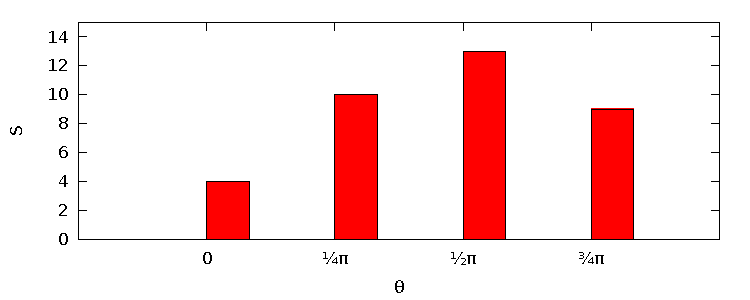
\includegraphics[width=0.45\textwidth]{img/steerable}
\caption{Example image -- Coastal Sunset, 1990-2006}\label{fig:example-img}
\end{figure}

\begin{figure}[h]
\centering
% GNUPLOT: LaTeX picture
\setlength{\unitlength}{0.240900pt}
\ifx\plotpoint\undefined\newsavebox{\plotpoint}\fi
\sbox{\plotpoint}{\rule[-0.200pt]{0.400pt}{0.400pt}}%
\begin{picture}(900,540)(0,0)
\sbox{\plotpoint}{\rule[-0.200pt]{0.400pt}{0.400pt}}%
\put(171.0,131.0){\rule[-0.200pt]{4.818pt}{0.400pt}}
\put(151,131){\makebox(0,0)[r]{ 0}}
\put(819.0,131.0){\rule[-0.200pt]{4.818pt}{0.400pt}}
\put(171.0,205.0){\rule[-0.200pt]{4.818pt}{0.400pt}}
\put(151,205){\makebox(0,0)[r]{ 20}}
\put(819.0,205.0){\rule[-0.200pt]{4.818pt}{0.400pt}}
\put(171.0,278.0){\rule[-0.200pt]{4.818pt}{0.400pt}}
\put(151,278){\makebox(0,0)[r]{ 40}}
\put(819.0,278.0){\rule[-0.200pt]{4.818pt}{0.400pt}}
\put(171.0,352.0){\rule[-0.200pt]{4.818pt}{0.400pt}}
\put(151,352){\makebox(0,0)[r]{ 60}}
\put(819.0,352.0){\rule[-0.200pt]{4.818pt}{0.400pt}}
\put(171.0,425.0){\rule[-0.200pt]{4.818pt}{0.400pt}}
\put(151,425){\makebox(0,0)[r]{ 80}}
\put(819.0,425.0){\rule[-0.200pt]{4.818pt}{0.400pt}}
\put(171.0,499.0){\rule[-0.200pt]{4.818pt}{0.400pt}}
\put(151,499){\makebox(0,0)[r]{ 100}}
\put(819.0,499.0){\rule[-0.200pt]{4.818pt}{0.400pt}}
\put(305.0,131.0){\rule[-0.200pt]{0.400pt}{4.818pt}}
\put(305,90){\makebox(0,0){$0$}}
\put(305.0,479.0){\rule[-0.200pt]{0.400pt}{4.818pt}}
\put(438.0,131.0){\rule[-0.200pt]{0.400pt}{4.818pt}}
\put(438,90){\makebox(0,0){$\frac{\pi}{4}$}}
\put(438.0,479.0){\rule[-0.200pt]{0.400pt}{4.818pt}}
\put(572.0,131.0){\rule[-0.200pt]{0.400pt}{4.818pt}}
\put(572,90){\makebox(0,0){$\frac{\pi}{2}$}}
\put(572.0,479.0){\rule[-0.200pt]{0.400pt}{4.818pt}}
\put(705.0,131.0){\rule[-0.200pt]{0.400pt}{4.818pt}}
\put(705,90){\makebox(0,0){$\frac{3\pi}{4}$}}
\put(705.0,479.0){\rule[-0.200pt]{0.400pt}{4.818pt}}
\put(171.0,131.0){\rule[-0.200pt]{0.400pt}{88.651pt}}
\put(171.0,131.0){\rule[-0.200pt]{160.921pt}{0.400pt}}
\put(839.0,131.0){\rule[-0.200pt]{0.400pt}{88.651pt}}
\put(171.0,499.0){\rule[-0.200pt]{160.921pt}{0.400pt}}
\put(30,315){\makebox(0,0){$S$}}
\put(505,29){\makebox(0,0){$\theta$}}
\put(305.0,131.0){\rule[-0.200pt]{0.400pt}{3.613pt}}
\put(305.0,146.0){\rule[-0.200pt]{10.600pt}{0.400pt}}
\put(349.0,131.0){\rule[-0.200pt]{0.400pt}{3.613pt}}
\put(305.0,131.0){\rule[-0.200pt]{10.600pt}{0.400pt}}
\put(438.0,131.0){\rule[-0.200pt]{0.400pt}{8.913pt}}
\put(438.0,168.0){\rule[-0.200pt]{10.840pt}{0.400pt}}
\put(483.0,131.0){\rule[-0.200pt]{0.400pt}{8.913pt}}
\put(438.0,131.0){\rule[-0.200pt]{10.840pt}{0.400pt}}
\put(572.0,131.0){\rule[-0.200pt]{0.400pt}{11.563pt}}
\put(572.0,179.0){\rule[-0.200pt]{10.600pt}{0.400pt}}
\put(616.0,131.0){\rule[-0.200pt]{0.400pt}{11.563pt}}
\put(572.0,131.0){\rule[-0.200pt]{10.600pt}{0.400pt}}
\put(705.0,131.0){\rule[-0.200pt]{0.400pt}{7.950pt}}
\put(705.0,164.0){\rule[-0.200pt]{10.840pt}{0.400pt}}
\put(750.0,131.0){\rule[-0.200pt]{0.400pt}{7.950pt}}
\put(705.0,131.0){\rule[-0.200pt]{10.840pt}{0.400pt}}
\put(171.0,131.0){\rule[-0.200pt]{0.400pt}{88.651pt}}
\put(171.0,131.0){\rule[-0.200pt]{160.921pt}{0.400pt}}
\put(839.0,131.0){\rule[-0.200pt]{0.400pt}{88.651pt}}
\put(171.0,499.0){\rule[-0.200pt]{160.921pt}{0.400pt}}
\end{picture}

\caption{Steerable filter strength $S(\theta)$ on the example image in figure~\ref{fig:example-img}}
\end{figure}

Gabor filters are linear filters which can be tuned to a greater range of
angles and frequencies than simple steerable filters, which in turn results in
a more accurate representation of the texture of the painting. The general
equation for a Gabor filter is given in Equation~\ref{gabor_eq}.

\begin{equation}
g_e(x) = \frac{1}{2\pi\sigma_x \sigma_y}e^{-\frac{1}{2}\left(\frac{x^2}{\sigma_x}+\frac{y^2}{\sigma_y}\right)}\cos(2\pi\omega_{x_0}x + 2\pi\omega_{y_0}y)
\label{gabor_eq}
\end{equation}

Where $(\omega_{x_0},\omega_{y_0})$\ defines the centre frequency, and
$(\sigma_x,\sigma_y)$ the spread of the Gaussian window. In this work we use
Gabor filters tuned to equally spaced orientations to build a histogram
representing line orientations in each painting, and present results below for
histograms built from the output of both 4 and 8 filter orientations.

\textbf{XXX Hannah or Alex to look at a textbook for a better version of the above scary maths and cite.}

\textbf{XXX Alex to run Gabor with 4 and 8.}

The final method for producing histograms we consider involves the application
of two discrete derivative masks to the image to get the gradient of $x$ and
$y$, and then to work out the gradient direction at each point. These gradient
directions are then summarised in a histogram of oriented gradients, providing
a yet richer representation of the texture of the image. This is similar to the
method described in \cite{Dalal2005Histograms}. 

\textbf{XXX Alex we use 15 bins; can we try different bin size? or is that just
me being fussy? It'd be good to have Gabor (4, 8, 16); HOG (4, 8, 16); thus
providing a direct comparator}

% Right oh now what we need is some graphs
% I suggest for now doing results in-line, or have a table here showing 
% correlation coefficients 

% \textbf{Alex is going to combine the various correlation-against-K graphs so that we have one graph with all techniques on the same axes}

\section{Year classification results}
\label{results}

\begin{figure}[h]
\centering
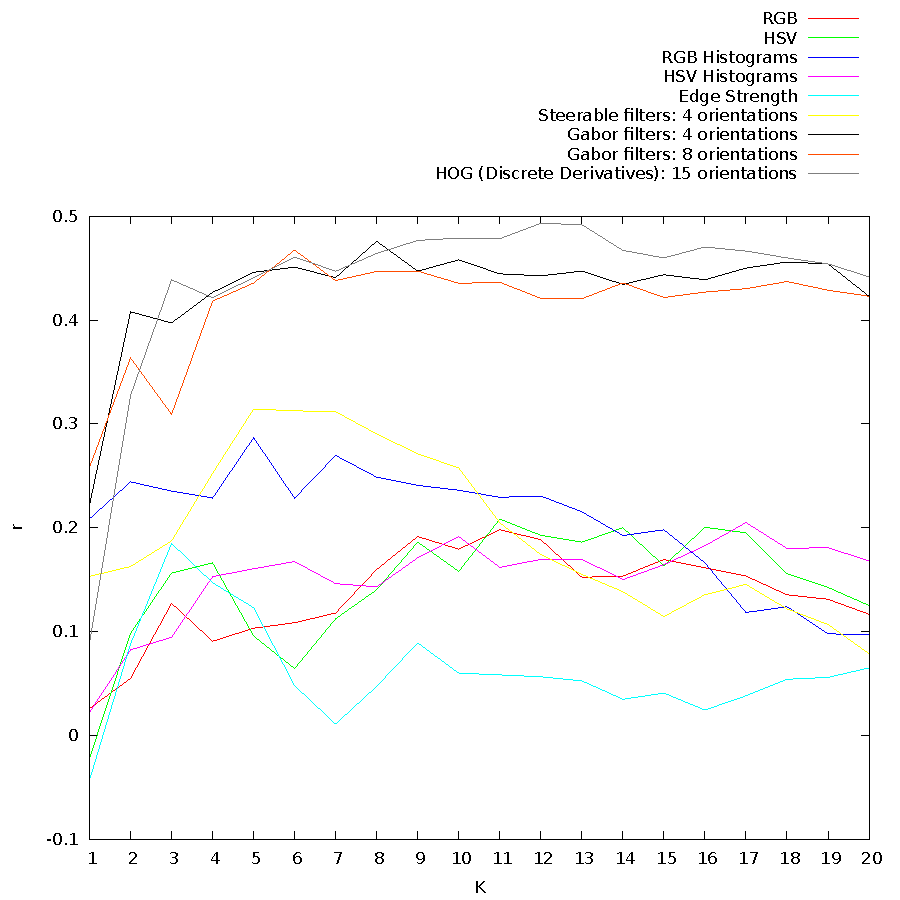
\includegraphics[width=0.5\textwidth]{results/mean.pdf}
\label{pearsons-k}
%% GNUPLOT: LaTeX picture using EEPIC macros
\setlength{\unitlength}{0.120450pt}
\begin{picture}(3000,1800)(0,0)
\footnotesize
\thicklines \path(349,265)(390,265)
\thicklines \path(2876,265)(2835,265)
\put(308,265){\makebox(0,0)[r]{-0.1}}
\thicklines \path(349,410)(390,410)
\thicklines \path(2876,410)(2835,410)
\put(308,410){\makebox(0,0)[r]{ 0}}
\thicklines \path(349,555)(390,555)
\thicklines \path(2876,555)(2835,555)
\put(308,555){\makebox(0,0)[r]{ 0.1}}
\thicklines \path(349,701)(390,701)
\thicklines \path(2876,701)(2835,701)
\put(308,701){\makebox(0,0)[r]{ 0.2}}
\thicklines \path(349,846)(390,846)
\thicklines \path(2876,846)(2835,846)
\put(308,846){\makebox(0,0)[r]{ 0.3}}
\thicklines \path(349,991)(390,991)
\thicklines \path(2876,991)(2835,991)
\put(308,991){\makebox(0,0)[r]{ 0.4}}
\thicklines \path(349,1136)(390,1136)
\thicklines \path(2876,1136)(2835,1136)
\put(308,1136){\makebox(0,0)[r]{ 0.5}}
\thicklines \path(349,265)(349,306)
\thicklines \path(349,1136)(349,1095)
\put(349,182){\makebox(0,0){ 1}}
\thicklines \path(482,265)(482,306)
\thicklines \path(482,1136)(482,1095)
\put(482,182){\makebox(0,0){ 2}}
\thicklines \path(615,265)(615,306)
\thicklines \path(615,1136)(615,1095)
\put(615,182){\makebox(0,0){ 3}}
\thicklines \path(748,265)(748,306)
\thicklines \path(748,1136)(748,1095)
\put(748,182){\makebox(0,0){ 4}}
\thicklines \path(881,265)(881,306)
\thicklines \path(881,1136)(881,1095)
\put(881,182){\makebox(0,0){ 5}}
\thicklines \path(1014,265)(1014,306)
\thicklines \path(1014,1136)(1014,1095)
\put(1014,182){\makebox(0,0){ 6}}
\thicklines \path(1147,265)(1147,306)
\thicklines \path(1147,1136)(1147,1095)
\put(1147,182){\makebox(0,0){ 7}}
\thicklines \path(1280,265)(1280,306)
\thicklines \path(1280,1136)(1280,1095)
\put(1280,182){\makebox(0,0){ 8}}
\thicklines \path(1413,265)(1413,306)
\thicklines \path(1413,1136)(1413,1095)
\put(1413,182){\makebox(0,0){ 9}}
\thicklines \path(1546,265)(1546,306)
\thicklines \path(1546,1136)(1546,1095)
\put(1546,182){\makebox(0,0){ 10}}
\thicklines \path(1679,265)(1679,306)
\thicklines \path(1679,1136)(1679,1095)
\put(1679,182){\makebox(0,0){ 11}}
\thicklines \path(1812,265)(1812,306)
\thicklines \path(1812,1136)(1812,1095)
\put(1812,182){\makebox(0,0){ 12}}
\thicklines \path(1945,265)(1945,306)
\thicklines \path(1945,1136)(1945,1095)
\put(1945,182){\makebox(0,0){ 13}}
\thicklines \path(2078,265)(2078,306)
\thicklines \path(2078,1136)(2078,1095)
\put(2078,182){\makebox(0,0){ 14}}
\thicklines \path(2211,265)(2211,306)
\thicklines \path(2211,1136)(2211,1095)
\put(2211,182){\makebox(0,0){ 15}}
\thicklines \path(2344,265)(2344,306)
\thicklines \path(2344,1136)(2344,1095)
\put(2344,182){\makebox(0,0){ 16}}
\thicklines \path(2477,265)(2477,306)
\thicklines \path(2477,1136)(2477,1095)
\put(2477,182){\makebox(0,0){ 17}}
\thicklines \path(2610,265)(2610,306)
\thicklines \path(2610,1136)(2610,1095)
\put(2610,182){\makebox(0,0){ 18}}
\thicklines \path(2743,265)(2743,306)
\thicklines \path(2743,1136)(2743,1095)
\put(2743,182){\makebox(0,0){ 19}}
\thicklines \path(2876,265)(2876,306)
\thicklines \path(2876,1136)(2876,1095)
\put(2876,182){\makebox(0,0){ 20}}
\thicklines \path(349,1136)(349,265)(2876,265)(2876,1136)(349,1136)
\put(61,700){\makebox(0,0)[l]{\shortstack{$r$}}}
\put(1612,58){\makebox(0,0){$K$}}
\put(2589,1718){\makebox(0,0)[r]{RGB Colour-Space Analysis}}
\thinlines \path(2630,1718)(2835,1718)
\thinlines \path(349,448)(349,448)(482,490)(615,595)(748,542)(881,560)(1014,568)(1147,581)(1280,642)(1413,688)(1546,670)(1679,697)(1812,684)(1945,631)(2078,633)(2211,656)(2344,644)(2477,633)(2610,607)(2743,600)(2876,579)
\put(2589,1635){\makebox(0,0)[r]{HSV Colour-Space Analysis}}
\thicklines \path(2630,1635)(2835,1635)
\thicklines \path(349,378)(349,378)(482,553)(615,637)(748,651)(881,549)(1014,503)(1147,573)(1280,614)(1413,680)(1546,639)(1679,712)(1812,690)(1945,680)(2078,700)(2211,647)(2344,701)(2477,693)(2610,636)(2743,617)(2876,592)
\put(2589,1552){\makebox(0,0)[r]{RGB Histogram Analysis}}
\Thicklines \path(2630,1552)(2835,1552)
\Thicklines \path(349,713)(349,713)(482,764)(615,752)(748,742)(881,826)(1014,742)(1147,801)(1280,771)(1413,759)(1546,753)(1679,743)(1812,745)(1945,723)(2078,689)(2211,697)(2344,651)(2477,582)(2610,590)(2743,552)(2876,551)
\put(2589,1469){\makebox(0,0)[r]{HSV Histogram Analysis}}
\thinlines \path(2630,1469)(2835,1469)
\thinlines \path(349,442)(349,442)(482,530)(615,547)(748,632)(881,643)(1014,653)(1147,622)(1280,618)(1413,658)(1546,688)(1679,645)(1812,656)(1945,656)(2078,628)(2211,649)(2344,675)(2477,708)(2610,672)(2743,672)(2876,654)
\put(2589,1386){\makebox(0,0)[r]{Edge Strength Analysis}}
\thicklines \path(2630,1386)(2835,1386)
\thicklines \path(349,347)(349,347)(482,538)(615,679)(748,623)(881,589)(1014,480)(1147,426)(1280,478)(1413,539)(1546,497)(1679,495)(1812,492)(1945,486)(2078,460)(2211,469)(2344,445)(2477,465)(2610,488)(2743,491)(2876,504)
\put(2589,1303){\makebox(0,0)[r]{Histogram of Oritenated Gradients Analysis}}
\Thicklines \path(2630,1303)(2835,1303)
\Thicklines \path(349,539)(349,539)(482,885)(615,1047)(748,1022)(881,1050)(1014,1079)(1147,1059)(1280,1084)(1413,1102)(1546,1105)(1679,1104)(1812,1126)(1945,1124)(2078,1088)(2211,1078)(2344,1093)(2477,1087)(2610,1078)(2743,1069)(2876,1051)
\thicklines \path(349,1136)(349,265)(2876,265)(2876,1136)(349,1136)
\end{picture}

\caption{Correlation Coefficients $r$ against K values for K-Nearest Neighbour}
\end{figure}

% you're not going to like me for this but can you plot the other feature
%spaces too?

The one parameter of our classifier is the choice of K in K-nearest neighbour.
Simply setting $K=1$\ has the effect of assigning the year of the nearest
painting in feature space to the current test painting, whereas setting
$K=102$\ has the effect of giving each painting the mean value of the entire
dataset. Clearly a point between these two extremes would be best; from
Figure~\ref{pearsons-k} we can see that for many of the feature spaces we
consider, the optimum K value is around 7 or 8.

\textbf{XXX Alex - can we get the results table for K=7?}

\begin{table}[h]
\centering
\begin{tabular}{|p{3.5cm}|c|c|}
\hline
Technique     & $r$ & $P(r)$ \\ \hline
Edge Strength & 0.060 & 0.52877 \\
HSV           & 0.158 & 0.09518 \\
RGB           & 0.179 & 0.05757 \\
HSV Histogram & 0.364 & 0.00007 \\
Steerable filters: 4 orientations & & \\
Gabor filters: 4 orientations & & \\
Gabor filters: 8 orientations & & \\
HOG (Discrete Derivatives): 15 orientations & 0.479 & 0.00000008 \\
\hline
\end{tabular}
\vspace{0.5em}
\caption{Correlation Coefficients, ordered by strength}\label{tab:results}
\end{table}

\textbf{XXX Alex - do we have HOG results for steerable, Gabor, and derivative masks?}

\textbf{XXX Alex - do we have any ensemble methods? IIRC combining HOG with HSV gave us impressive correlations}

\section{Exemplars: can we improve results by incorporating expert knowledge? }

We have also investigated the utility of incorporating expert knowledge within
our framework. For each year represented in our collection we asked Dr Paul
Joyner, of the National Library of Wales, to choose the one painting which best
represents the artist's work for that year. Dr Joyner is a member of the
Trustees of the Kyffin Williams Estate and he has written widely on Welsh Art
and Kyffin Williams. These chosen paintings we consider to be
connoisseurially/artistically selected exemplars (\emph{artistic exemplars}, for
short), which we can then use as a representation of that particular year.

The data on artistic exemplars opens up the options for different methods of
classification. Rather than using K-nearest neighbour to classify each point in
the feature space, we can take the year of the nearest exemplar to assign that year
to the painting in question. 

This then raises the question of whether we can determine \emph{statistical
exemplars} to compare with our \emph{artistic exemplars}, and if so what the
digitally-chosen exemplars would be.  We can either use cluster centres (which
provides us with a point in feature space which will not correspond to an
actual painting), or the nearest actual painting to the feature space centroid
for a year. The former technique does not, strictly speaking, give us an
exemplar; the latter chooses as exemplar the painting which best represents a
particular year according to a particular feature space. 

\textbf{XXX Alex - We need results:-)}

\textbf{XXX Alex again - can we get an indication of any situations where our statistic exemplars match the artistic ones, and the converse situation (artistic exemplars nowhere near centres of feature space)? This is a good place for us to include a couple of extra photos of paintings}

\subsection{Comparing Artistic and Statistical Exemplars}

The same distance measure used to run k-nearest neighbour on the feature-based classifiers was
used to generate the error between the statistical and artistic exemplars.

%TODO I need to actually write some more code for this

\textbf{XXX Alex... er... your to do list is longer than mine:-)}

\section{Conclusions and future directions}

To the best of our knowledge this is the first work that attempts to date work
by an artist by year. Similarly, we believe we are the first to try and perform
digital analysis of paintings from a range of catalogue and web images. The
results presented here show that computer vision \emph{can} help with the job
of dating art within an artist's body of work. 

Future directions will involve testing the methods presented here on the works
of other artists who have shown great stylistic variation over the course of
their career: we would like to build a dataset of, for example, David Hockney
works.  Whilst we have not yet performed this test we are hopeful of success;
by avoiding brushstroke detection (which we expect to be artist specific) we
hope to have developed techniques with application across a broader range of
artistic styles. 



% conference papers do not normally have an appendix


% use section* for acknowledgement
\section*{Acknowledgment}


The authors would like to thank Dr Paul Joyner of the National Library of Wales
for his invaluable expert assistance. We would also like to thank Professor
Robert Meyrick of the School of Art, Aberystywth University.





% trigger a \newpage just before the given reference
% number - used to balance the columns on the last page
% adjust value as needed - may need to be readjusted if
% the document is modified later
%\IEEEtriggeratref{8}
% The "triggered" command can be changed if desired:
%\IEEEtriggercmd{\enlargethispage{-5in}}

% references section

% can use a bibliography generated by BibTeX as a .bbl file
% BibTeX documentation can be easily obtained at:
% http://www.ctan.org/tex-archive/biblio/bibtex/contrib/doc/
% The IEEEtran BibTeX style support page is at:
% http://www.michaelshell.org/tex/ieeetran/bibtex/
\bibliographystyle{IEEEtran}
% argument is your BibTeX string definitions and bibliography database(s)
\bibliography{references}

% that's all folks
\end{document}
